
\chapter{Principe Physique}

\label{lab:chapPET}
La Tomographie par \'Emission de Positons (TEP) est une modalité d'imagerie fonctionnelle utilisant la désintégration d'un traceur radioactif pour mettre en valeur les zones de forte activité métaboliques. Elle est principalement utilisée en imagerie cérébrale, oncologie et cardiologie.


	\section{Généralités}

L'imagerie TEP permet de visualiser de manière indirecte des processus physiologiques survenant dans le corps du patient. Je vais présenter rapidement les évènements qui se produisent lors d'un examen, présentés dans la figure \ref{fig:schemaTEP}.

Pour cela, on lui injecte un ``traceur'' contenant une particule radioactive. Ce traceur est conçu de manière à se fixer sur les zones du corps que l'on souhaite imager. Pendant toute la durée de l'examen, les particules radioactives vont se désintégrer selon la loi de décroissance radioactive de la formule \ref{eq:loidecradioact}.

\begin{equation}
	dN = - \lambda N dt
	\label{eq:loidecradioact}
\end{equation}

$N$ représente le nombre le particules radioactives présentes dans le corps du patient. $dN$ représente la variation de ce nombre de particules (le nombre de désintégrations par $dt$) et $\lambda$ est une constante dépendant de l'élément radioactif.

Chaque désintégration d'un élément radioactif va déclencher l'émission d'une particule chargée $\beta^+$, aussi appellée positon. En oncologie, on utilise le Fluor $^{18}F$ qui se désintégre en Oxygène $^{18}O$ en émettant le positon. Cette particule va parcourir quelques mm avant de s'annihiler avec un élection en émettant 2 photons dans deux directions opposées avec une énergie de 511 KeV.

Ce seront ces photons qui vont être détectés par l'imageur TEP. Ils représentent une coïncidence, car l'instant d'arrivée et leur énergie sont semblables. L'ensemble des ``Lignes de réponse'' (LDR) correspondant aux coïncidences détectées est utilisée pour reconstruire les images.

\begin{figure}
\centering
\includegraphics[width=16cm]{images/schemaTEP}
\caption[Présentation simplifiée de la TEP]{Processus d'un examen TEP : a) Injection du traceur radioactif, qui va se fixer préférentiellement sur les zones que l'on cherche à observer. b) Désintégration d'un atome radioactif du traceur, ici dans la zone à imager. Cela entraîne l'émission de deux photons dans deux directions opposées, qui seront détectés dans la couronne de capteurs. c) Tous les évènements détectés sont stockés dans la mémoire de la console, ici sous forme de sinogramme. d) L'image est reconstruite à la suite de l'acquisition pour former un volume 3D estimant la répartition du traceur dans l'organisme.}
\label{fig:schemaTEP}
\end{figure}

	\subsection{\'Emission des photons}

Nous allons maintenant détailler le processus qui déclenche l'émission des photons détectés par l'imageur, présenté dans la figure~\ref{fig:Langner2008ad}.

Les émetteurs de positons utilisés en TEP sont des isotopes radioactifs présentant un excès de charge positive, ou proton, dans leurs noyaux. Un processus de désintégration $\beta^+$, correspondant à la transformation d’un proton $p$ en un neutron $n$, leur permet de migrer vers un état stable. Cette désintégration résulte en l’émission d’un neutrino $\nu$ et d’un positron $e^+$ selon l’équation \ref{eq:desinteg}. Le positron est une particule de même masse que l’électron mais de charge opposée.

\begin{equation}
 p~\rightarrow~n + e^+ + \nu
\label{eq:desinteg}
\end{equation}

Le positon va alors s'annihiler avec un électron après un parcours de quelques millimètres en émettant deux photons de même énergie (511 keV) comme indiqué dans l'équation~\ref{eq:annihilation}. L'angle d'émission des photons est approximé en supposant qu'ils sont émis à $180°$ l'un de l'autre, alors qu'en réalité il existe une incertitude de $\pm 0.25°$~\cite{bailey2005positron}.

\begin{equation}
 e^+ + e^-~\rightarrow~\gamma + \gamma
\label{eq:annihilation}
\end{equation}

\begin{figure}
\centering
\includegraphics[width=12cm]{images/annihilation}
\caption[\'Emission des photons]{\'Emission des photons~\cite{Langner2008ad} : Le radiotraceur de désintègre en émettant un neutrino et un positron. Après un parcours de quelques mm dans les tissus, ce dernier s'annihile avec un électron. Cette réaction provoque la création de deux photons d'énergie 511 keV partant dans deux directions opposées.}
\label{fig:Langner2008ad}
\end{figure}

	\subsection{Détection des photons}

Les détecteurs utilisés en TEP sont constitués d'un matériau photomultiplicateur placé devant un photodetecteur. Chaque photon absorbé par le matériau photomultiplicateur va entraîner une réaction en chaîne qui qui va déclencher une émission lumineuse. Le capteur situé derrière va convertir cette émission lumineuse en charge électrique.

Un système électronique placé à proximité de l'imageur va ensuite apparier les photons détectés pour retrouver la ligne de réponse (LDR) sur laquelle la désintégration a eu lieu. les paires de photon assemblées correspondent à des coïncidence.

Les coïncidences vraies Figure \ref{fig:schemaDetections}(a) correspondent aux cas où les deux détections appairées correspondent bien à une seule désintégration et où aucun des photons n'a été dévié. Les coïncidences fortuites Figure \ref{fig:schemaDetections}(b) correspondent à deux désintégrations simultanées qui sont considérées comme étant une seule désintégration. Enfin, les coïncidences diffusées Figure \ref{fig:schemaDetections}(c) sont le résultat de la déviation d'un des deux photons produit. Pour éliminer ces erreurs, un certains nombre de méthodes ont été implémentées, dont le filtrage en énergie et en temps au niveau matériel : ne sont prises en compte que les paires d'évènements arrivant dans une fenêtre temporelle et énergétique définie. En effet, les photons déviés vont perdre de l'énergie, ce qui va entraîner leur élimination.

\begin{figure}
\centering
\includegraphics[width=12cm]{images/schemaDetections}
\caption[Les différents types de coïncidences en TEP]{Les différents types de coïncidences en TEP. Le trajet réel du photon est indiqué en trait fin simple, tandis que la ligne de réponse est indiquée en trait pointillé épais. On appelle les coïncidences vraies (a) lorsque l'annihilation est bien sur la ligne de réponse, fortuites (b) lorsque deux désintégrations réalisées en même temps sont considérées comme une seule et diffusée (c) lorsqu'un des photons est dévié.}
\label{fig:schemaDetections}
\end{figure}



	\section{perturbation trajet du photon}

Les deux interactions les plus importantes que peuvent avoir les photons avec les tissus sont la diffusion compton et l'absorption photoélectrique.

La diffusion compton corresponds à l'interaction entre le photon émis et un électron du milieu. L'énergie cinétique de l'électron sera augmentée, tandis que le photon sera dévié. Il est intéressant de noter qu'une déviation de 25° engendre une perte d'énergie du photon de seulement 10\%~\cite{evans1955atomic}.

L'absorbtion photo-électrique correspond quand à elle à l'interaction entre un noyau atomique et un des photon. L'énergie du photon sera absorbré par le noyau et transmis à un de ses électrons. Cet effet est praticulièrement important en TEP, car il génère des artefacts très visibles, qui doivent être corrigés à partir d'une carte d'atténuation, déduite d'un examen de Tomodensitométrie (Tomographie par rayons X) ou d'une carte de transmission, comme indiqué en~\ref{fig:schemaAtt}.

L'atténuation augmente exponentiellement avec la longueur du trajet dans les tissus selon la loi de Beer-Lambert :
\begin{equation}
I = I_0 e^{-\mu l}
\end{equation}

Avec $I_0$ la quantité originale de photons, $I$ le nombre de photons qui traverseront le milieu, $\mu$ le coefficient d'atténuation du milieu et $l$ la longueur du trajet. 

Dans le cas où le milieu est complexe, et si l'on connaît l'atténuation $\mu(x)$ en chaque point $x$ du trajet :

\begin{equation}
I = I_0 e^{- \int\limits^L_0 \mu(l) dl}
\end{equation}



\begin{figure}
\centering
\includegraphics[width=12cm]{images/attenuationNonAtt}
\caption[Effet de l'atténuation sur les images TEP]{Effets de l'atténuation sur des images TEP : L'image de gauche correspond à la distribution de radioactivité reçue par les détecteurs. On peu observer une perte progressive de l'activité vers l'intérieur des tissus, cars le photons on plus de chances d'intéragir avec la matière. L'image TDM au centre est utilisée pour estimer l'atténuation des tissus et prendre en compte cette atténuation lors de la reconstruction de l'image de droite.}
\label{fig:schemaAtt}
\end{figure}


\chapter{Déroulement d'une acquisition}

Nous allons maintenant décrire répidement quelques points techniques permettant de mieux comprendre comment sont réalisées les acquisitions. Nous y parlerons de la méthode utilisée pour réaliser des acquisitions corps entier alors que l'imageur a un champ de vue faible et des contraintes associées, mais aussi du format des données et de ce que cela implique.

	\section{Acquisitions corps entier}


Les acquisitions TEP réalisées pour l'oncologie sont habituellement des acquisitions corps entier, de manière à pouvoir avoir une vue de l'étendue des lésions.

Or le champ de vue axial d'une caméra TEP est de quelques centimètres seulement (18 cm pour le Philips Gemini GXL). En routine clinique, les patients sont placés sur des lits qui se déplacent par incréments successifs lors de l'acquisition.

Le nombre de lits est déterminé par la taille du patient ainsi que par le champ de vue du tomographe. Chaque lit est reconstruit séparément puis assemblé avec les lits suivants et précédents, comme indiqué dans la figure \ref{fig:multilits}. \'Etant donné que les caméra TEP ont une sensibilité plus faible à leur extrémités, on introduit un chevauchement plus ou moins important dans les lits.

\begin{figure}
\centering
\includegraphics[width=12cm]{images/multilits}
\caption[Acquisitions corps entier en TEP]{Réalisation d'une acquisition corps entier en TEP : Chaque lit est acquis et reconstruit séparément avec un chevauchement. Les lits sont ensuite assemblés pour produire l'image finale.}
\label{fig:multilits}
\end{figure}

Les acquisitions corps entier utilisent typiquement 6 à 7 lits pour une caméra siemens, ce qui demande un temps considérable. Il faut donc faire des compromis entre le temps d'acquisition et la qualité des images. Sachant que les examens TEP sont coûteux et que l'immobilité est inconfortable pour les patients, le temps d'acquisition est calibré pour durer moins d'une heure au total. Les nouvelles génération d'imageurs permettent cependant de réduire les temps d'acquisition à qualité équivalente.

	\section{Acquisition en mode 2D ou 3D}

Historiquement, les données étaient acquises par coupe : des septas (plaque destinées à absorber les photons) étaient placés entre les détecteur de manière à éliminer les photons qui n'étaient pas émis dans le plan (voir figure \ref{fig:2D3D}. De la même manière, les coïncidences étaient recherchées par plan uniquement.

Cependant, bien que le nombre de coïncidences fortuites est peu élevé suite à la réduction du flux de photons, la quantité de données acquise est plus faible, ce qui a amené aux acquisitions 3D, où les septas sont retirés et où les photons peuvent être détectés selon des angles plus larges.


\begin{figure}
\centering
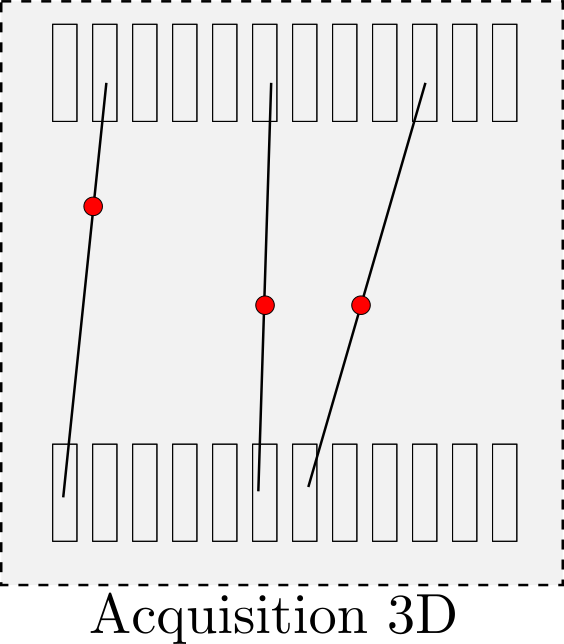
\includegraphics[width=12cm]{images/2D3D}
\caption[Acquisitions 2D et 3D en TEP]{Illustration des différences entre l'acquisition 2D et 3D en TEP. Les deux images représentent un imageur vu en coupe axiale. les rectangles blancs représentent les détecteurs et les rectangles noirs les septas destinés à bloquer les photons. }
\label{fig:2D3D}
\end{figure}


	\section{Corrections de l'atténuation}

\label{CorrectionAttenuation}

Le patient passe tout d'abord un exament TDM sur les scanner couplés TEP/TDM. Les valeurs des coefficients hounsfield correspondant à l'atténuation des rayons X sont transformés pour correspondre à l'atténuation des photons de 511keV de la TEP. Ce sera cette image qui sera utilisée pour réaliser la correction d'atténuation. 

Il est cependant possible d'utiliser une image en transmission, où une source radioactive est placé dans l'imageur et tourne autour du patient. L'activité de la source étant connue, la quantité de photons reçue par les détecteur situés derrière le patient permet de générer la carte d'atténuation du corps du patient, de la même manière que pour l'imagerie TDM. Cependant, la généralisation des scanner couplées TEP/TDM limite l'utilisation de cette technique.



Lors de l'appariment des photons, 


	\section{Format des données}
Les données acquises par une caméra TEP peuvent être stockées sous deux formes principales : Sinogramme et séquentiel.
		\subsection{Séquentiel}

Ce format correspond à un enregistrement ``brut'' des données issues de l'électronique de la caméra.

Ce format de fichier est en fait un enregistrement séquentiel des évènements, dans leur ordre de détection. On peut enregistrer chaque photon détecté indépendamment, ou encore uniquement les coïncidences. Chaque évènement est daté, ce qui permet de conserver l'informations temporelle, qui est utilisé notamment pour synchroniser les données acquises avec le temps, pour la correction de mouvement par exemple.

Il existe plusieurs formats de fichiers pour le stockage de ces données, notamment le format LMF (List-Mode Format) développé pour le projet ClearPET et le format ROOT développé par le CERN. 

L'avantage de ces formats est qu'ils permettent de conserver les informations sur la dynamique de l'acquisition, mais aussi qu'ils permettent le stockage de métadonnées utiles en simulations, notamment le nombre de diffusions, ou de marquer les coincidences fortuites.

Cependant ce format consomme une très grande quantité de mémoire, étant donné qu'un examen PET est constitué de plusieurs millions d'évènements.

		\subsection{Sinogramme}

Le sinogramme est une matrice indiquant pour chaque ligne de réponse le nombre de détections réalisées. Dans le cas d'acquisitions en mode 2D, où chaque coupe est séparée des autres par un blindage, on empile typiquement les sinogrammes des coupes. Dans le mode 3D, le blindage est retiré, ce qui permet de détecter des paires de photon qui ne sont pas directement dans le plan du détecteur. Dans ce cas, une dimension supplémentaire est ajoutée pour prendre en compte cet effet.

Le principal avantage du sinogramme est qu'il permet de stocker les données acquises lors d'un examen TEP de manière beaucoup plus compacte que le format séquentiel. Cependant, il ne conserve aucune information temporelle.


\chapter{Algorithmes de reconstruction}

La reconstruction des images TEP corresponds à un problème inverse : à partir de l'ensemble des lignes de réponse, il faut déduire la répartition du radiotraceur dans l'organisme du patient. Deux classes d'algorithme existent pour résoudre ce type de problèmes, mais actuellement seul les algorithmes itératifs sont utilisés en oncologie clinique. 

	\section{Itératifs}

La relation liant l'image TEP $f$ et les projections sur les détecteurs $p$ est la suivante :

\begin{equation}
	p = R f + n
\end{equation}

Avec $H$ la matrice de projection et $n$ les erreurs provenant des erreurs dans les données. On considère que les comptages des lignes de réponses $p_i$ sont indépendants et bruités selon une loi de poisson. Ce problèmes est mal posé, et nécessite donc l'utilisation d'algorithmes spécialisés. 

Des techniques existent pour corriger les données des effets vu dans la figure \ref{fig:schemaDetections}, notamment l'implantation d'une ligne à retard pour estimer les coïncidences aléatoires puis les retirer du sinogramme.

		\subsection{Maximum Likelihood Expectation Maximisation (ML-EM) }


L'algorithme ML-EM est initialisé avec une image de départ $f_0$. Il se déroule en deux phases principales : une phase de comparaison de l'image au niveau $n$ avec les lignes de réponses observées, puis une phase de mise à jour de l'image pour prendre en compte les différences calculées à l'étape précédente, comme présenté dans la figure \ref{fig:schemaMLEM}.

En pratique, la matrice de $H$ correspond à la matrice vu $R$ précédemment mais inclus des informations supplémentaires pour corriger les différences de sensibilité entre les différents capteurs, mais aussi réaliser la correction des diffusés~\cite{shepp1982maximum,chornoboy1990evaluation}. Cette matrice peut aussi être utilisée pour corriger l'atténuation des tissus. En pratique, cette matrice ``système'' $H_ij$ indique la probabilité de détecter une désintégration au voxel $j$ de l'image dans la ligne de réponse $i$ :

\begin{equation}
	f_j^{(n+1)}=\frac{\hat{f}_j^{(n)}}{\sum\limits_{i'}H_{i'j}}\sum\limits_{i}H_{ij}\frac{p_i}{\sum\limits_{k}H_{ik}\hat{f}_k^{(n)}}
\label{eq:MLEM}
\end{equation}


Le nombre d'itérations à réaliser avant d'atteindre la convregence dépend de l'image, mais il est couramment d'environ 20 à 50. Il existe plusieurs publications proposant un critère d'arrêt~\cite{bissantz2006multi}, mais en pratique la reconstruction est souvent réalisée pour un nombre d'itérations fixées~\cite{bailey2005positron} et  suivi d'un filtrage passe-bas~\cite{daube2001application}. Cet algorithme de reconstruction prends un temps important car il faut réaliser l'opération de projection et de retroprojection sur l'ensemble des données à chaque itération.

\begin{figure}
\centering
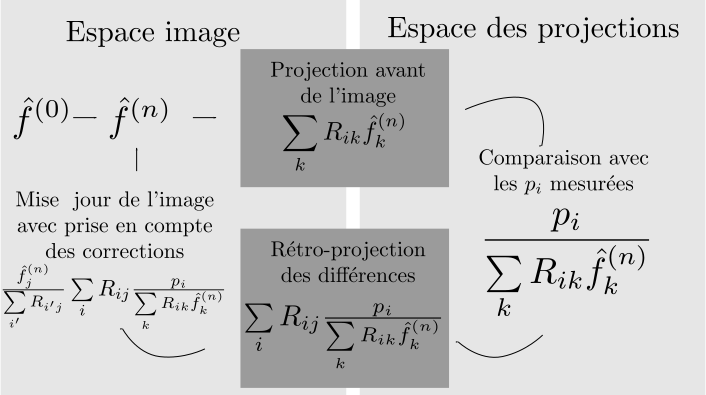
\includegraphics[width=12cm]{images/MLEM}
\caption[Schéma de principe de l'algorithme MLEM]{Schéma décrivant l'alorithme itératif ML-EM. $\hat{f}^{(n)}_j$ est l'estimation du voxel $j$ de l'image à l'itération $n$. $H_{ij}$ est la matrice système, et représente la probabilité de détecter une désintégration dans le voxel $j$ à la ligne de réponse $i$.}
\label{fig:schemaMLEM}
\end{figure}


	\subsection{Ordered Subset Expectation Maximisation (OS-EM)}

L'algorithme OS-EM est une évolution de l'algorithme ML-EM  qui permet une accélération substantielle de la convergence en réalisant les itérations de l'équation \ref{eq:MLEM} sur des sous-ensemble des données acquises~\cite{hudson1994accelerated}. 

Ces sous-ensemble de données sont réalisés en échantillonant de manière régulière les lignes de réponses. Leur nombre est un des paramètres de l'algorithme, mais la convergence n'est plus garantie contrairement à ML-EM. En pratique, l'image converge toujours, et un nombre pré-déterminé d'itérations est déterminé de manière empirique~\cite{bailey2005positron}. Des évolutions de OS-EM ont été réalisées pour garantir une convergence, notamment l'algorithme Row-Action Maximum Likelihood (RAMLA)~\cite{browne1996row, chiang2004clinical}.

Le principal avantage de OS-EM est qu'il permet d'augmenter la vitesse de la reconstruction d'un facteur correspondant au nombre de sous-ensembles utilisés.

	\subsection{Cas des acquisitions en mode Séquentiel}

Les acquisitions en mode séquentiel génèrent une suite d'enregistrements correspondant aux évènements détectés par l'imageur. Le parcours de tous ces évènements un par un demande des temps de calculs extrèmement importants, c'est pourquoi Reader~\cite{reader2002one} a proposé une adaptation de l'OS-EM au mode séquentiel appellée One-Pass List-Mode EM (OPL-EM). L'algorithme proposé est conçu pour ne parcourir qu'une seule fois la liste des évènements. Comme pour OS-EM, les données sont groupées en sous-ensemble, qui sont utilisés les uns après les autres pour chaque itération, comme indiqué dans la figure suivante :

\begin{equation}
	f_j^{(n+1)}=\frac{\hat{f}_j^{(n)}}{\sum\limits_{i'}H_{i'j}}\sum\limits_{i \in T^n}H_{ij}\frac{1}{\sum\limits_{k}H_{ik}\hat{f}_k^{(n)}}
\label{eq:OSEM_seq}
\end{equation}

La différence avec OS-EM est que la sommation des différences est réalisée sur l'ensemble d'avènements $T^n$ correspondant au sous-ensemble d'évènements associé à l'itération $n$. Cette somme est réalisée non pas pour chaque ligne de réponse $q_i$ comme précédemment, mais pour chaque évènement détecté, ce qui explique le remplacement par la valeur 1.
		
	\section{Analytiques}

Les reconstructions analytiques utilisent le théorème de la coupe centrale pour réaliser la rétroprojection de données. Ce théorème permet de lier les transformée de fourier des projections avec celles de l'image d'origine. 
 
Ces algorithmes sont supplantés en oncologie par les algorithmes itératifs qui sont jugés plus performants sur l'évaluation du SUV et moins bruités~\cite{schoder2004clinical}.